\documentclass[12pt,a4paper]{article}

% Packages
\usepackage{geometry}
\geometry{margin=1in}
\usepackage{fancyhdr}
\usepackage{titlesec}
\usepackage{listings}
\usepackage{xcolor}
\usepackage{graphicx}

% Header & Footer
\pagestyle{fancy}
\fancyhf{}
\rhead{DBT - Assignment 2}
\lhead{Kamithkar Vinod}
\cfoot{\thepage}

% Title formatting
\titleformat{\section}{\large\bfseries}{Problem \thesection:}{0.5em}{}
\titleformat{\subsection}[runin]{\bfseries}{Code:}{0.5em}{}[---]
\titleformat{\subsubsection}[runin]{\bfseries}{Output:}{0.5em}{}[---]

% SQL language definition for listings
\lstdefinelanguage{SQL}{
  morekeywords={
    SELECT, FROM, WHERE, GROUP, BY, ORDER, ASC, DESC, JOIN, ON, AS,
    AND, OR, NOT, IN, IS, NULL, LIKE, HAVING, COUNT, SUM, AVG, MIN, MAX,
    CREATE, TABLE, INSERT, INTO, VALUES, UPDATE, SET, DELETE, DISTINCT,
    CASE, WHEN, THEN, ELSE, END, BETWEEN, EXISTS, UNION, ALL, ANY, LEFT,
    RIGHT, INNER, OUTER, LIMIT, OFFSET
  },
  sensitive=false,
  morecomment=[l]{--},
  morestring=[b]',
}

\lstset{
    language=SQL,
    basicstyle=\ttfamily\small,
    keywordstyle=\color{blue}\bfseries,
    commentstyle=\color{gray}\itshape,
    stringstyle=\color{red},
    showstringspaces=false,
    frame=single,
    breaklines=true,
    numbers=none
}

% Document Start
\begin{document}

% Title Page
\begin{center}
    \LARGE \textbf{Assignment - 2} \\[0.5cm]
    \Large \textbf{DBMS} \\[1cm]

    \begin{tabular}{rl}
        \textbf{Name:} & Kamithkar Vinod \\
        \textbf{Course:} & PG DAC AUGUST 2025 \\
        \textbf{PRN:} & 250850320040 \\
        \textbf{Form No:} & 250500480 \\
        \textbf{Date:} & 17-10-2025 \\
    \end{tabular}
\end{center}

\vspace{1cm}
\hrule
\vspace{0.5cm}

% Problems

% 1
\section{}
\textbf{Task:} Display each employee's name and hiredate from department 20.

\subsection{}
\begin{lstlisting}
SELECT ename, hiredate, deptno
FROM emp
WHERE deptno = 20;
\end{lstlisting}

\subsubsection{}
\begin{center}
    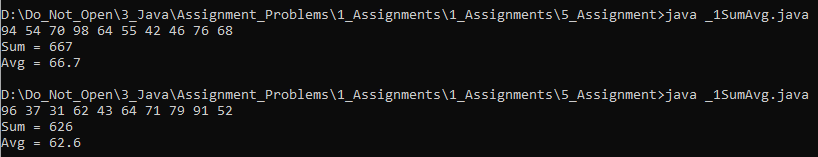
\includegraphics[width=0.8\textwidth]{1.png}
\end{center}

% 2

\section{}
\textbf{Task:} Display each employee's name with hiredate and salary review date.
Assume review date is one year after hiredate.

\subsection{}
\begin{lstlisting}
SELECT ename,
       hiredate,
       DATE_ADD(hiredate, INTERVAL 1 YEAR) AS "Salary Review Date"
FROM emp;
\end{lstlisting}

\subsubsection{}
\begin{center}
    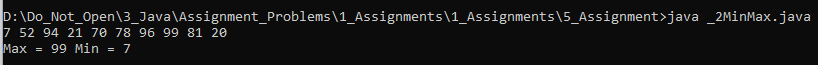
\includegraphics[width=0.8\textwidth]{2.png}
\end{center}

% 3

\section{}
\textbf{Task:} Print a list of employees displaying just salary if more than 1500. If
exactly 1500 then display 'On Target', if less than 1500 then display
'Below 1500'.

\subsection{}
\begin{lstlisting}
SELECT ename,
       sal,
       CASE
         WHEN sal = 1500 THEN 'On Target'
         WHEN sal < 1500 THEN 'Below 1500'
         ELSE CAST(sal AS CHAR)
       END AS status
FROM emp;
\end{lstlisting}

\subsubsection{}
\begin{center}
    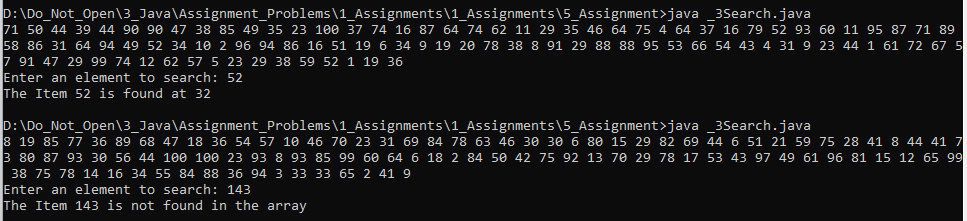
\includegraphics[width=0.8\textwidth]{3.png}
\end{center}

% 4

\section{}
\textbf{Task:} Find the minimum salary of all employees.

\subsection{}
\begin{lstlisting}
SELECT MIN(sal) AS Min_Salary
FROM emp;
\end{lstlisting}

\subsubsection{}
\begin{center}
    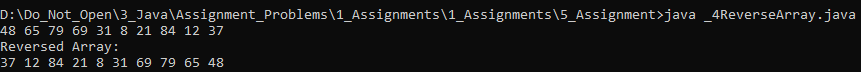
\includegraphics[width=0.8\textwidth]{4.png}
\end{center}

% 5

\section{}
\textbf{Task:} Find the minimum, maximum and average salaries of all employees.

\subsection{}
\begin{lstlisting}
SELECT MIN(sal) AS Min_Salary,
       MAX(sal) AS Max_Salary,
       AVG(sal) AS Avg_Salary
FROM emp;
\end{lstlisting}

\subsubsection{}
\begin{center}
    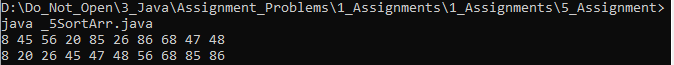
\includegraphics[width=0.8\textwidth]{5.png}
\end{center}

% 6

\section{}
\textbf{Task:} List the minimum and maximum salary for each job type.

\subsection{}
\begin{lstlisting}
SELECT job,
       MIN(sal) AS Min_Salary,
       MAX(sal) AS Max_Salary
FROM emp
GROUP BY job;
\end{lstlisting}

\subsubsection{}
\begin{center}
    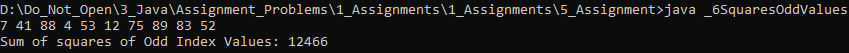
\includegraphics[width=0.8\textwidth]{6.png}
\end{center}

% 7

\section{}
\textbf{Task:} Find out the average salary and total remuneration for each job type.

\subsection{}
\begin{lstlisting}
SELECT job,
       AVG(sal) AS Avg_Salary,
       SUM(sal + IFNULL(comm, 0)) AS Total_Remuneration
FROM emp
GROUP BY job;
\end{lstlisting}

\subsubsection{}
\begin{center}
    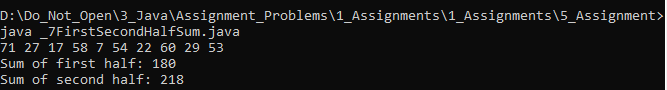
\includegraphics[width=0.8\textwidth]{7.png}
\end{center}

% 8

\section{}
\textbf{Task:} Find out the difference between highest and lowest salaries.

\subsection{}
\begin{lstlisting}
SELECT MIN(sal) AS Min_Salary,
       MAX(sal) AS Max_Salary,
       (MAX(sal) - MIN(sal)) AS Difference
FROM emp;
\end{lstlisting}

\subsubsection{}
\begin{center}
    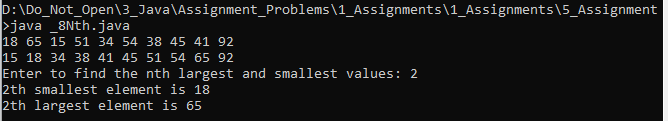
\includegraphics[width=0.8\textwidth]{8.png}
\end{center}

% 9

\section{}
\textbf{Task:} Find all departments, which have more than 3 employees.

\subsection{}
\begin{lstlisting}
SELECT deptno,
       COUNT(*) AS Employee_Count
FROM emp
GROUP BY deptno
HAVING COUNT(*) > 3;
\end{lstlisting}

\subsubsection{}
\begin{center}
    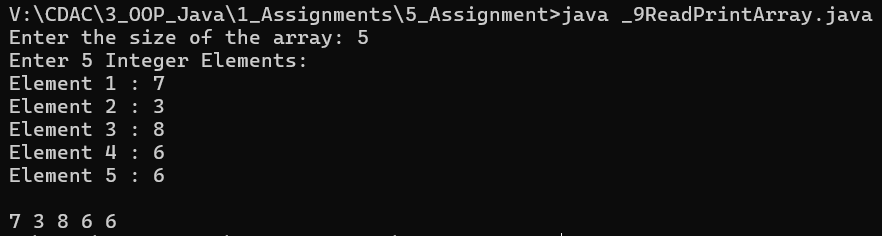
\includegraphics[width=0.8\textwidth]{9.png}
\end{center}

% 10

\section{}
\textbf{Task:} Check whether all employee numbers are indeed unique.

\subsection{}
\begin{lstlisting}
SELECT empno,
       COUNT(*) AS cnt
FROM emp
GROUP BY empno
HAVING COUNT(*) > 1;
\end{lstlisting}

\subsubsection{}
\begin{center}
    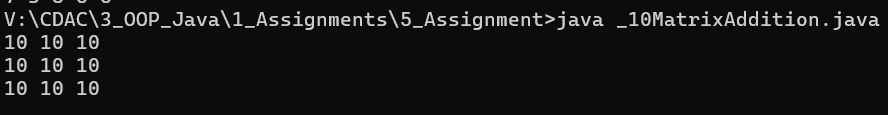
\includegraphics[width=0.8\textwidth]{10.png}
\end{center}

% 11

\section{}
\textbf{Task:} List the lowest paid employees working for each manager. Exclude any
groups where the minimum salary is less than 1000. Sort the output by
salary.

\subsection{}
\begin{lstlisting}
SELECT e.mgr,
       e.empno,
       e.ename,
       e.sal
FROM emp e
JOIN (
    SELECT mgr, MIN(sal) AS min_sal
    FROM emp
    GROUP BY mgr
    HAVING MIN(sal) >= 1000
) m ON e.mgr = m.mgr AND e.sal = m.min_sal
ORDER BY e.sal;
\end{lstlisting}

\subsubsection{}
\begin{center}
    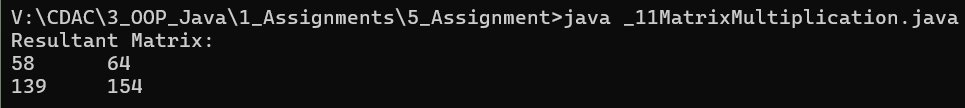
\includegraphics[width=0.8\textwidth]{11.png}
\end{center}

% 12

\section{}
\textbf{Task:} Display all employee names and their department names, in the order of
department name.

\subsection{}
\begin{lstlisting}
SELECT e.ename,
       d.dname
FROM emp e
JOIN dept d ON e.deptno = d.deptno
ORDER BY d.dname;
\end{lstlisting}

\subsubsection{}
\begin{center}
    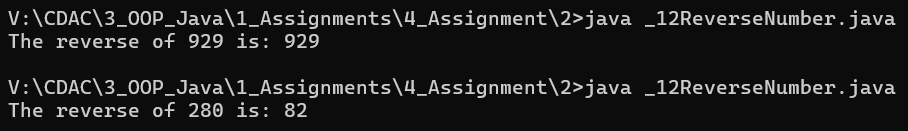
\includegraphics[width=0.8\textwidth]{12.png}
\end{center}

% 13

\section{}
\textbf{Task:} Display all employee names, department number and department name.

\subsection{}
\begin{lstlisting}
SELECT e.ename,
       d.deptno,
       d.dname
FROM emp e
JOIN dept d ON e.deptno = d.deptno;
\end{lstlisting}

\subsubsection{}
\begin{center}
    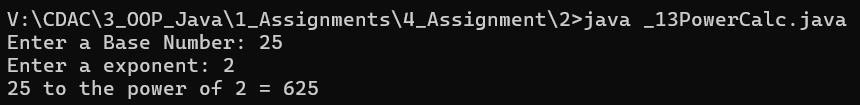
\includegraphics[width=0.8\textwidth]{13.png}
\end{center}

% 14

\section{}
\textbf{Task:} Display the name, location and department of employees whose salary is
more than 1500 a month.

\subsection{}
\begin{lstlisting}
SELECT e.ename,
       d.loc,
       d.dname
FROM emp e
JOIN dept d ON e.deptno = d.deptno
WHERE e.sal > 1500;
\end{lstlisting}

\subsubsection{}
\begin{center}
    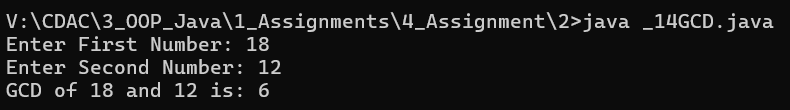
\includegraphics[width=0.8\textwidth]{14.png}
\end{center}

% 15

\section{}
\textbf{Task:} Show only employees on grade 3.

\subsection{}
\begin{lstlisting}
SELECT e.ename,
       e.sal,
       s.grade
FROM emp e
JOIN salgrade s ON e.sal BETWEEN s.losal AND s.hisal
WHERE s.grade = 3;
\end{lstlisting}

\subsubsection{}
\begin{center}
    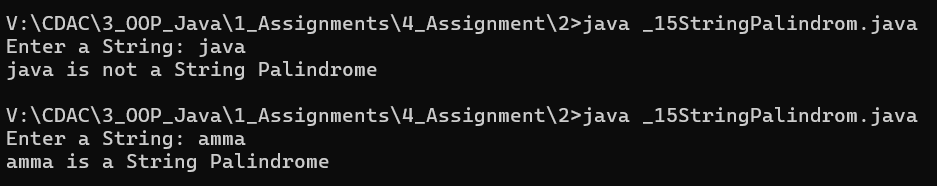
\includegraphics[width=0.8\textwidth]{15.png}
\end{center}

% 16

\section{}
\textbf{Task:} Show all employees in 'Dallas'.

\subsection{}
\begin{lstlisting}
SELECT *
FROM emp
WHERE deptno = (
    SELECT deptno
    FROM dept
    WHERE loc = 'Dallas'
);
\end{lstlisting}

\subsubsection{}
\begin{center}
    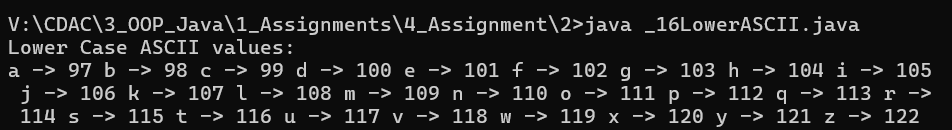
\includegraphics[width=0.8\textwidth]{16.png}
\end{center}

% 17

\section{}
\textbf{Task:} List the employee name, job, salary, and grade and department name for
everyone in the company except clerks. Sort on salary, displaying the
salary first.

\subsection{}
\begin{lstlisting}
SELECT e.sal  AS Salary,
       e.ename AS Employee_Name,
       e.job   AS Job,
       s.grade AS Grade,
       d.dname AS Department_Name
FROM emp e
JOIN dept d ON e.deptno = d.deptno
JOIN salgrade s ON e.sal BETWEEN s.losal AND s.hisal
WHERE UPPER(e.job) <> 'CLERK'
ORDER BY e.sal;
\end{lstlisting}

\subsubsection{}
\begin{center}
    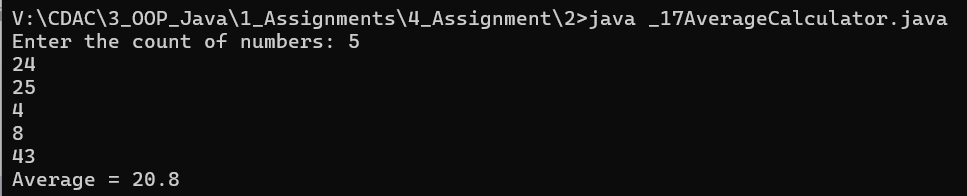
\includegraphics[width=0.8\textwidth]{17.png}
\end{center}

% 18

\section{}
\textbf{Task:} List the details of employees who earn 36000 a year or who are clerks.

\subsection{}
\begin{lstlisting}
SELECT *
FROM emp
WHERE (sal * 12) = 36000
   OR UPPER(job) = 'CLERK';
\end{lstlisting}

\subsubsection{}
\begin{center}
    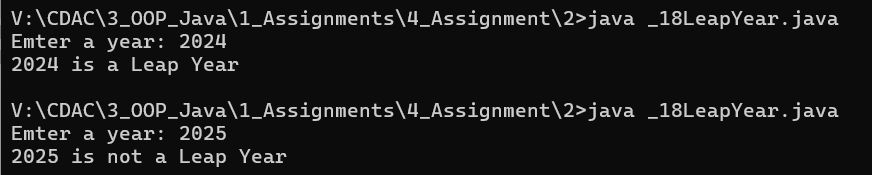
\includegraphics[width=0.8\textwidth]{18.png}
\end{center}

% 19

\section{}
\textbf{Task:} Display the department that has no employees.

\subsection{}
\begin{lstlisting}
SELECT dname
FROM dept
WHERE deptno NOT IN (SELECT DISTINCT deptno FROM emp);
\end{lstlisting}

\subsubsection{}
\begin{center}
    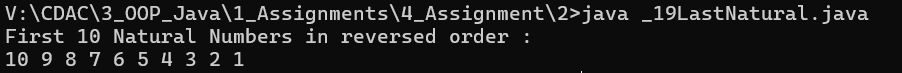
\includegraphics[width=0.8\textwidth]{19.png}
\end{center}

% 20

\section{}
\textbf{Task:} Find the employees who earn the highest salary in each job type. Sort in
descending salary order.

\subsection{}
\begin{lstlisting}
SELECT e.job,
       e.ename,
       e.sal
FROM emp e
WHERE e.sal = (
    SELECT MAX(sal)
    FROM emp
    WHERE job = e.job
)
ORDER BY e.sal DESC;
\end{lstlisting}

\subsubsection{}
\begin{center}
    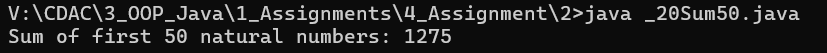
\includegraphics[width=0.8\textwidth]{20.png}
\end{center}

% 21

\section{}
\textbf{Task:} Find the most recently hired employees in each department ordered by
hire date.

\subsection{}
\begin{lstlisting}
SELECT e.deptno,
       e.ename,
       e.hiredate
FROM emp e
WHERE e.hiredate = (
    SELECT MAX(hiredate)
    FROM emp
    WHERE deptno = e.deptno
)
ORDER BY e.hiredate DESC;
\end{lstlisting}

\subsubsection{}
\begin{center}
    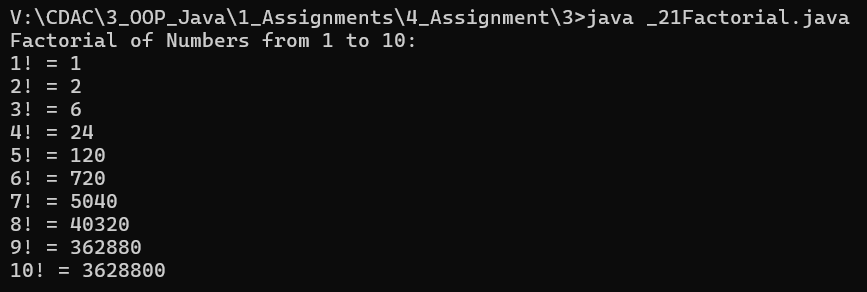
\includegraphics[width=0.8\textwidth]{21.png}
\end{center}

% 22

\section{}
\textbf{Task:} Display the details of employees hired between Jan and June.

\subsection{}
\begin{lstlisting}
-- Works in Oracle / DBs supporting TO_CHAR; for MySQL use MONTH(hiredate) BETWEEN 1 AND 6
SELECT *
FROM emp
WHERE TO_CHAR(hiredate, 'MM') BETWEEN '01' AND '06';
\end{lstlisting}

\subsubsection{}
\begin{center}
    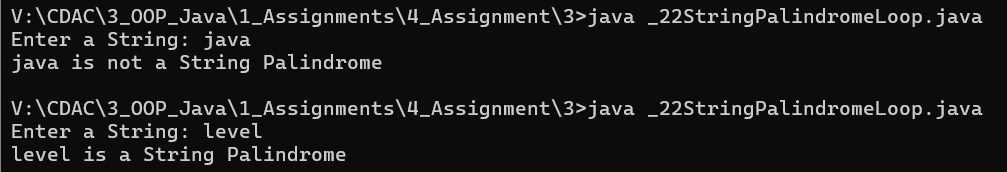
\includegraphics[width=0.8\textwidth]{22.png}
\end{center}

% 23

\section{}
\textbf{Task:} Display the count, total salary and average salary of all employees in each
department.

\subsection{}
\begin{lstlisting}
SELECT deptno,
       COUNT(*) AS Emp_Count,
       SUM(sal) AS Total_Salary,
       AVG(sal) AS Average_Salary
FROM emp
GROUP BY deptno;
\end{lstlisting}

\subsubsection{}
\begin{center}
    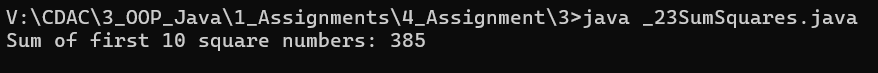
\includegraphics[width=0.8\textwidth]{23.png}
\end{center}

% 24

\section{}
\textbf{Task:} Find a square root of the number 36.1111. The result should not contain
any decimal spaces.

\subsection{}
\begin{lstlisting}
-- Round the square root to nearest integer (no decimals)
SELECT ROUND(SQRT(36.1111)) AS Square_Root
FROM dual;
\end{lstlisting}

\subsubsection{}
\begin{center}
    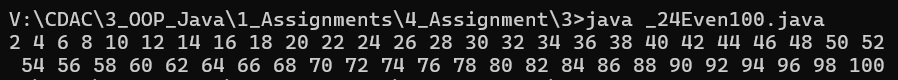
\includegraphics[width=0.8\textwidth]{24.png}
\end{center}

% 25

\section{}
\textbf{Task:} Given a string 'HELLO_THERE_'. Replace all '_' with '!' marks.

\subsection{}
\begin{lstlisting}
SELECT REPLACE('HELLO_THERE_', '_', '!') AS NEW_STRING
FROM dual;
\end{lstlisting}

\subsubsection{}
\begin{center}
    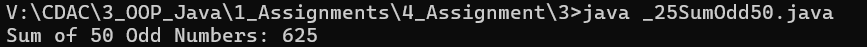
\includegraphics[width=0.8\textwidth]{25.png}
\end{center}

% 26

\section{}
\textbf{Task:} Find the sum of the length of the strings. The String are CDAC,
HYDERABAD.

\subsection{}
\begin{lstlisting}
SELECT LENGTH('CDAC') + LENGTH('HYDERABAD') AS Total_Length
FROM dual;
\end{lstlisting}

\subsubsection{}
\begin{center}
    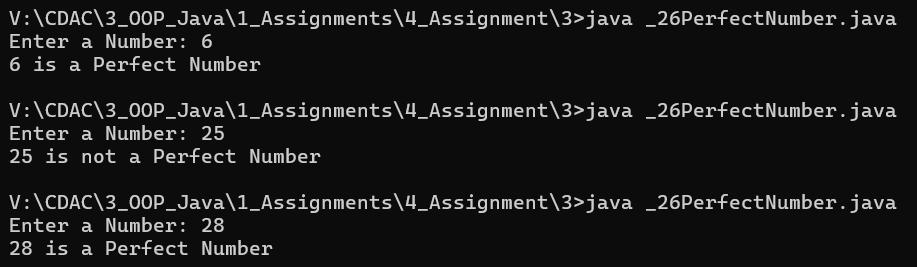
\includegraphics[width=0.8\textwidth]{26.png}
\end{center}

% 27

\section{}
\textbf{Task:} Find the job that was filled in the first half of the 1980 and the job that
was filled during the same period in 1981.

\subsection{}
\begin{lstlisting}
SELECT job, hiredate
FROM emp
WHERE (TO_CHAR(hiredate, 'YYYY') = '1980' AND TO_CHAR(hiredate, 'MM') BETWEEN '01' AND '06')
   OR (TO_CHAR(hiredate, 'YYYY') = '1981' AND TO_CHAR(hiredate, 'MM') BETWEEN '01' AND '06');
\end{lstlisting}

\subsubsection{}
\begin{center}
    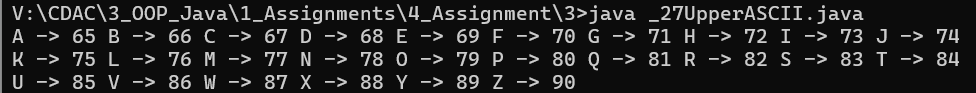
\includegraphics[width=0.8\textwidth]{27.png}
\end{center}

\end{document}
